\documentclass[twoside]{book}

% Packages required by doxygen
\usepackage{calc}
\usepackage{doxygen}
\usepackage{graphicx}
\usepackage[utf8]{inputenc}
\usepackage{makeidx}
\usepackage{multicol}
\usepackage{multirow}
\usepackage{fixltx2e}
\PassOptionsToPackage{warn}{textcomp}
\usepackage{textcomp}
\usepackage[nointegrals]{wasysym}
\usepackage[table]{xcolor}

% Font selection
\usepackage[T1]{fontenc}
\usepackage{mathptmx}
\usepackage[scaled=.90]{helvet}
\usepackage{courier}
\usepackage{amssymb}
\usepackage{sectsty}
\renewcommand{\familydefault}{\sfdefault}
\allsectionsfont{%
  \fontseries{bc}\selectfont%
  \color{darkgray}%
}
\renewcommand{\DoxyLabelFont}{%
  \fontseries{bc}\selectfont%
  \color{darkgray}%
}
\newcommand{\+}{\discretionary{\mbox{\scriptsize$\hookleftarrow$}}{}{}}

% Page & text layout
\usepackage{geometry}
\geometry{%
  a4paper,%
  top=2.5cm,%
  bottom=2.5cm,%
  left=2.5cm,%
  right=2.5cm%
}
\tolerance=750
\hfuzz=15pt
\hbadness=750
\setlength{\emergencystretch}{15pt}
\setlength{\parindent}{0cm}
\setlength{\parskip}{0.2cm}
\makeatletter
\renewcommand{\paragraph}{%
  \@startsection{paragraph}{4}{0ex}{-1.0ex}{1.0ex}{%
    \normalfont\normalsize\bfseries\SS@parafont%
  }%
}
\renewcommand{\subparagraph}{%
  \@startsection{subparagraph}{5}{0ex}{-1.0ex}{1.0ex}{%
    \normalfont\normalsize\bfseries\SS@subparafont%
  }%
}
\makeatother

% Headers & footers
\usepackage{fancyhdr}
\pagestyle{fancyplain}
\fancyhead[LE]{\fancyplain{}{\bfseries\thepage}}
\fancyhead[CE]{\fancyplain{}{}}
\fancyhead[RE]{\fancyplain{}{\bfseries\leftmark}}
\fancyhead[LO]{\fancyplain{}{\bfseries\rightmark}}
\fancyhead[CO]{\fancyplain{}{}}
\fancyhead[RO]{\fancyplain{}{\bfseries\thepage}}
\fancyfoot[LE]{\fancyplain{}{}}
\fancyfoot[CE]{\fancyplain{}{}}
\fancyfoot[RE]{\fancyplain{}{\bfseries\scriptsize Generated on Wed May 21 2014 21\+:31\+:42 for xilgame by Doxygen }}
\fancyfoot[LO]{\fancyplain{}{\bfseries\scriptsize Generated on Wed May 21 2014 21\+:31\+:42 for xilgame by Doxygen }}
\fancyfoot[CO]{\fancyplain{}{}}
\fancyfoot[RO]{\fancyplain{}{}}
\renewcommand{\footrulewidth}{0.4pt}
\renewcommand{\chaptermark}[1]{%
  \markboth{#1}{}%
}
\renewcommand{\sectionmark}[1]{%
  \markright{\thesection\ #1}%
}

% Indices & bibliography
\usepackage{natbib}
\usepackage[titles]{tocloft}
\setcounter{tocdepth}{3}
\setcounter{secnumdepth}{5}
\makeindex

% Hyperlinks (required, but should be loaded last)
\usepackage{ifpdf}
\ifpdf
  \usepackage[pdftex,pagebackref=true]{hyperref}
\else
  \usepackage[ps2pdf,pagebackref=true]{hyperref}
\fi
\hypersetup{%
  colorlinks=true,%
  linkcolor=blue,%
  citecolor=blue,%
  unicode%
}

% Custom commands
\newcommand{\clearemptydoublepage}{%
  \newpage{\pagestyle{empty}\cleardoublepage}%
}


%===== C O N T E N T S =====

\begin{document}

% Titlepage & ToC
\hypersetup{pageanchor=false,
             bookmarks=true,
             bookmarksnumbered=true,
             pdfencoding=unicode
            }
\pagenumbering{roman}
\begin{titlepage}
\vspace*{7cm}
\begin{center}%
{\Large xilgame }\\
\vspace*{1cm}
{\large Generated by Doxygen 1.8.7}\\
\vspace*{0.5cm}
{\small Wed May 21 2014 21:31:42}\\
\end{center}
\end{titlepage}
\clearemptydoublepage
\tableofcontents
\clearemptydoublepage
\pagenumbering{arabic}
\hypersetup{pageanchor=true}

%--- Begin generated contents ---
\chapter{Hierarchical Index}
\section{Class Hierarchy}
This inheritance list is sorted roughly, but not completely, alphabetically\+:\begin{DoxyCompactList}
\item \contentsline{section}{Board}{\pageref{class_board}}{}
\item \contentsline{section}{Cell}{\pageref{class_cell}}{}
\item \contentsline{section}{Display}{\pageref{class_display}}{}
\begin{DoxyCompactList}
\item \contentsline{section}{Display\+N\+Curses}{\pageref{class_display_n_curses}}{}
\item \contentsline{section}{Display\+Xil}{\pageref{class_display_xil}}{}
\end{DoxyCompactList}
\item \contentsline{section}{Drawing}{\pageref{class_drawing}}{}
\item \contentsline{section}{Iic\+Ctrl}{\pageref{class_iic_ctrl}}{}
\item \contentsline{section}{struct\+\_\+vres\+\_\+timing\+\_\+t}{\pageref{structstruct__vres__timing__t}}{}
\end{DoxyCompactList}

\chapter{Class Index}
\section{Class List}
Here are the classes, structs, unions and interfaces with brief descriptions\+:\begin{DoxyCompactList}
\item\contentsline{section}{\hyperlink{class_board}{Board} }{\pageref{class_board}}{}
\item\contentsline{section}{\hyperlink{class_cell}{Cell} }{\pageref{class_cell}}{}
\item\contentsline{section}{\hyperlink{class_display}{Display} }{\pageref{class_display}}{}
\item\contentsline{section}{\hyperlink{class_display_n_curses}{Display\+N\+Curses} }{\pageref{class_display_n_curses}}{}
\item\contentsline{section}{\hyperlink{class_display_xil}{Display\+Xil} }{\pageref{class_display_xil}}{}
\item\contentsline{section}{\hyperlink{class_drawing}{Drawing} }{\pageref{class_drawing}}{}
\item\contentsline{section}{\hyperlink{class_iic_ctrl}{Iic\+Ctrl} }{\pageref{class_iic_ctrl}}{}
\item\contentsline{section}{\hyperlink{structstruct__vres__timing__t}{struct\+\_\+vres\+\_\+timing\+\_\+t} }{\pageref{structstruct__vres__timing__t}}{}
\end{DoxyCompactList}

\chapter{Class Documentation}
\hypertarget{class_board}{\section{Board Class Reference}
\label{class_board}\index{Board@{Board}}
}
\subsection*{Public Member Functions}
\begin{DoxyCompactItemize}
\item 
\hypertarget{class_board_a1f0fa2da72d6b2b468429cf0958f8b78}{bool {\bfseries get\+State} (int, int)}\label{class_board_a1f0fa2da72d6b2b468429cf0958f8b78}

\item 
\hypertarget{class_board_a42e93605cefa1b1d704f9feb9879ac85}{void {\bfseries set\+Living\+Cell} (int, int)}\label{class_board_a42e93605cefa1b1d704f9feb9879ac85}

\item 
\hypertarget{class_board_aa9a9eaf138ff5af3869128188605d917}{void {\bfseries set\+Dead\+Cell} (int, int)}\label{class_board_aa9a9eaf138ff5af3869128188605d917}

\item 
\hypertarget{class_board_a81f1fb49a1d636a26540f6d9d5b100fb}{int {\bfseries num\+Living\+Neighbours} (int, int)}\label{class_board_a81f1fb49a1d636a26540f6d9d5b100fb}

\item 
\hypertarget{class_board_a62c179eb341c6b41bc89382f7a73da97}{void {\bfseries refresh\+Cell} (int, int)}\label{class_board_a62c179eb341c6b41bc89382f7a73da97}

\item 
\hypertarget{class_board_a76067c983fdc7641e3283d8d0699028c}{void {\bfseries refresh\+Board} (void)}\label{class_board_a76067c983fdc7641e3283d8d0699028c}

\item 
\hypertarget{class_board_a7fcb361b4c58c2ae650733d3d13a1202}{bool {\bfseries legal\+Column} (int)}\label{class_board_a7fcb361b4c58c2ae650733d3d13a1202}

\item 
\hypertarget{class_board_ad020f8b03af4e5b43f0d054f7c3fa2b3}{bool {\bfseries is\+Clear} (void)}\label{class_board_ad020f8b03af4e5b43f0d054f7c3fa2b3}

\end{DoxyCompactItemize}
\subsection*{Static Public Attributes}
\begin{DoxyCompactItemize}
\item 
\hypertarget{class_board_a4cd2277c8a8dbd23260f55d92abbf970}{static const int {\bfseries R\+O\+W\+\_\+\+S\+I\+Z\+E} = 50}\label{class_board_a4cd2277c8a8dbd23260f55d92abbf970}

\item 
\hypertarget{class_board_adfd96483c7ee6d2486c2b9b18b085fd0}{static const int {\bfseries C\+O\+L\+U\+M\+N\+\_\+\+S\+I\+Z\+E} = 100}\label{class_board_adfd96483c7ee6d2486c2b9b18b085fd0}

\end{DoxyCompactItemize}


The documentation for this class was generated from the following files\+:\begin{DoxyCompactItemize}
\item 
/\+Users/neiljohnson/sandbox/agile-\/codev-\/platform/sw/src/Board.\+h\item 
/\+Users/neiljohnson/sandbox/agile-\/codev-\/platform/sw/src/Board.\+cpp\end{DoxyCompactItemize}

\hypertarget{class_cell}{\section{Cell Class Reference}
\label{class_cell}\index{Cell@{Cell}}
}
\subsection*{Public Member Functions}
\begin{DoxyCompactItemize}
\item 
\hypertarget{class_cell_adc17181480ee0eece1b6e5e34d207dc7}{void {\bfseries set\+State} (bool)}\label{class_cell_adc17181480ee0eece1b6e5e34d207dc7}

\item 
\hypertarget{class_cell_ace7a562feab40550e990e8e637e3549d}{bool {\bfseries get\+State} (void)}\label{class_cell_ace7a562feab40550e990e8e637e3549d}

\item 
\hypertarget{class_cell_a40bf50831d93e983029a4a16261461a7}{bool {\bfseries is\+Alive} (int)}\label{class_cell_a40bf50831d93e983029a4a16261461a7}

\end{DoxyCompactItemize}


The documentation for this class was generated from the following files\+:\begin{DoxyCompactItemize}
\item 
/\+Users/neiljohnson/sandbox/agile-\/codev-\/platform/sw/src/Cell.\+h\item 
/\+Users/neiljohnson/sandbox/agile-\/codev-\/platform/sw/src/Cell.\+cpp\end{DoxyCompactItemize}

\hypertarget{class_display}{\section{Display Class Reference}
\label{class_display}\index{Display@{Display}}
}
Inheritance diagram for Display\+:\begin{figure}[H]
\begin{center}
\leavevmode
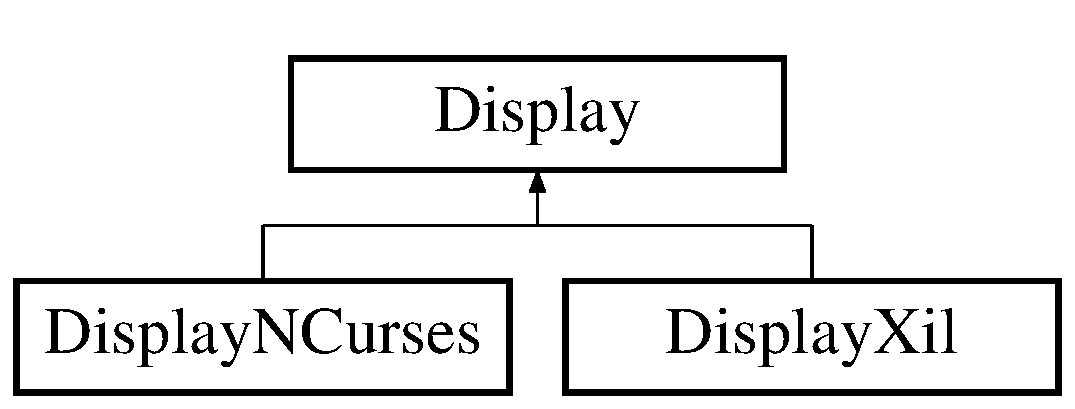
\includegraphics[height=2.000000cm]{class_display}
\end{center}
\end{figure}
\subsection*{Public Member Functions}
\begin{DoxyCompactItemize}
\item 
\hypertarget{class_display_a752a3b427cc86ef1afc35660e1083f61}{virtual int {\bfseries \+\_\+initscr} ()=0}\label{class_display_a752a3b427cc86ef1afc35660e1083f61}

\item 
\hypertarget{class_display_a8bd839f831135920320ec9df15dff4ea}{virtual void {\bfseries \+\_\+clear} ()=0}\label{class_display_a8bd839f831135920320ec9df15dff4ea}

\item 
\hypertarget{class_display_a8677bab55262fea0da3b7e10fa239eeb}{virtual void {\bfseries \+\_\+endwin} ()=0}\label{class_display_a8677bab55262fea0da3b7e10fa239eeb}

\item 
\hypertarget{class_display_a3af3e58e999e7a4bbe8747fef6a88c71}{virtual void {\bfseries \+\_\+refresh} ()=0}\label{class_display_a3af3e58e999e7a4bbe8747fef6a88c71}

\item 
\hypertarget{class_display_a5d6b10e388794156595f493f383a7068}{virtual void {\bfseries \+\_\+getch} ()=0}\label{class_display_a5d6b10e388794156595f493f383a7068}

\item 
\hypertarget{class_display_a5a9b0330abede469d35e294e5d5f5389}{virtual void {\bfseries \+\_\+addstr} (const char $\ast$)=0}\label{class_display_a5a9b0330abede469d35e294e5d5f5389}

\item 
\hypertarget{class_display_a6c5faed34fe0b7e386db82180134ff4f}{virtual void {\bfseries \+\_\+move} (int, int)=0}\label{class_display_a6c5faed34fe0b7e386db82180134ff4f}

\end{DoxyCompactItemize}


The documentation for this class was generated from the following files\+:\begin{DoxyCompactItemize}
\item 
/\+Users/neiljohnson/sandbox/agile-\/codev-\/platform/sw/src/Display.\+h\item 
/\+Users/neiljohnson/sandbox/agile-\/codev-\/platform/sw/src/Display.\+cpp\end{DoxyCompactItemize}

\hypertarget{class_display_n_curses}{\section{Display\+N\+Curses Class Reference}
\label{class_display_n_curses}\index{Display\+N\+Curses@{Display\+N\+Curses}}
}
Inheritance diagram for Display\+N\+Curses\+:\begin{figure}[H]
\begin{center}
\leavevmode
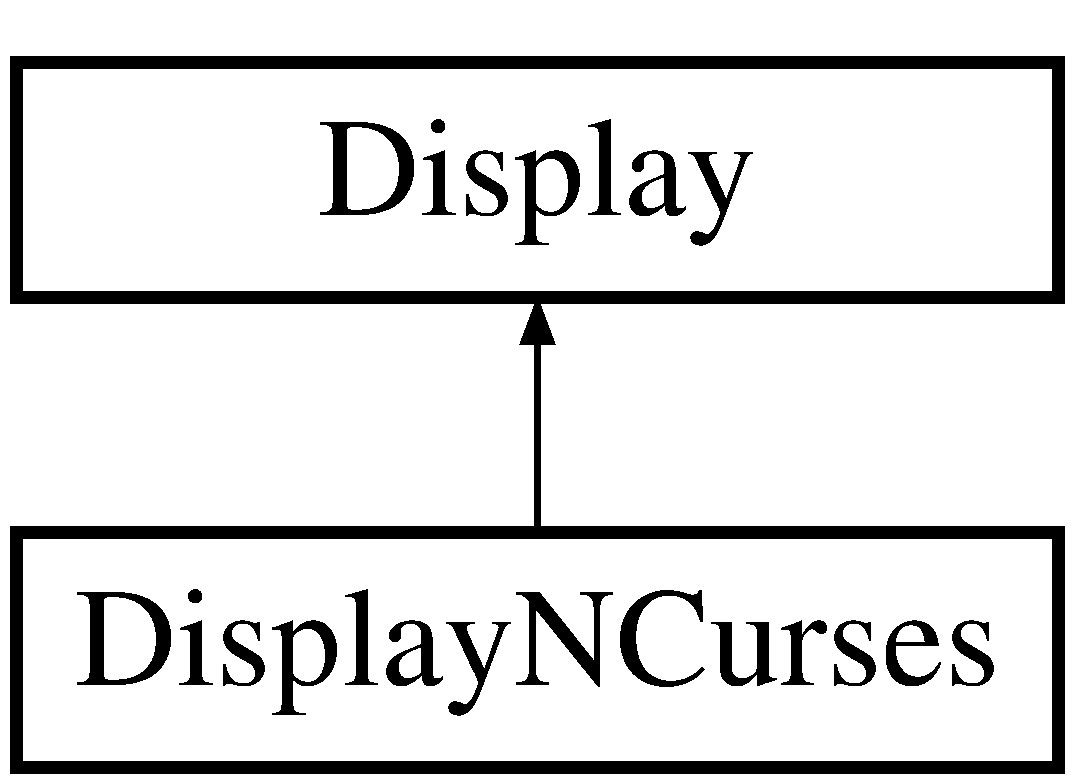
\includegraphics[height=2.000000cm]{class_display_n_curses}
\end{center}
\end{figure}
\subsection*{Public Member Functions}
\begin{DoxyCompactItemize}
\item 
\hypertarget{class_display_n_curses_a0cb29e78f2d3c19ef765739fc5481b23}{int {\bfseries \+\_\+initscr} ()}\label{class_display_n_curses_a0cb29e78f2d3c19ef765739fc5481b23}

\item 
\hypertarget{class_display_n_curses_a5874b9f4c6acc9d44c1de6813502bc31}{void {\bfseries \+\_\+clear} ()}\label{class_display_n_curses_a5874b9f4c6acc9d44c1de6813502bc31}

\item 
\hypertarget{class_display_n_curses_aab07a991fb72a70cabd8094d3b55cf5d}{void {\bfseries \+\_\+endwin} ()}\label{class_display_n_curses_aab07a991fb72a70cabd8094d3b55cf5d}

\item 
\hypertarget{class_display_n_curses_aa585c411a9b2e5e7d44903c7b86dbaa6}{void {\bfseries \+\_\+refresh} ()}\label{class_display_n_curses_aa585c411a9b2e5e7d44903c7b86dbaa6}

\item 
\hypertarget{class_display_n_curses_a0bddd32732caa6adf88c542ede448de9}{void {\bfseries \+\_\+getch} ()}\label{class_display_n_curses_a0bddd32732caa6adf88c542ede448de9}

\item 
\hypertarget{class_display_n_curses_a472957f2e0b2b2dcc056e5f1e741dc94}{void {\bfseries \+\_\+addstr} (const char $\ast$)}\label{class_display_n_curses_a472957f2e0b2b2dcc056e5f1e741dc94}

\item 
\hypertarget{class_display_n_curses_ab4ed85272039524b5a7273d7575d6aec}{void {\bfseries \+\_\+move} (int, int)}\label{class_display_n_curses_ab4ed85272039524b5a7273d7575d6aec}

\end{DoxyCompactItemize}


The documentation for this class was generated from the following files\+:\begin{DoxyCompactItemize}
\item 
/\+Users/neiljohnson/sandbox/agile-\/codev-\/platform/sw/src/Display\+N\+Curses.\+h\item 
/\+Users/neiljohnson/sandbox/agile-\/codev-\/platform/sw/src/Display\+N\+Curses.\+cpp\end{DoxyCompactItemize}

\hypertarget{class_display_xil}{\section{Display\+Xil Class Reference}
\label{class_display_xil}\index{Display\+Xil@{Display\+Xil}}
}
Inheritance diagram for Display\+Xil\+:\begin{figure}[H]
\begin{center}
\leavevmode
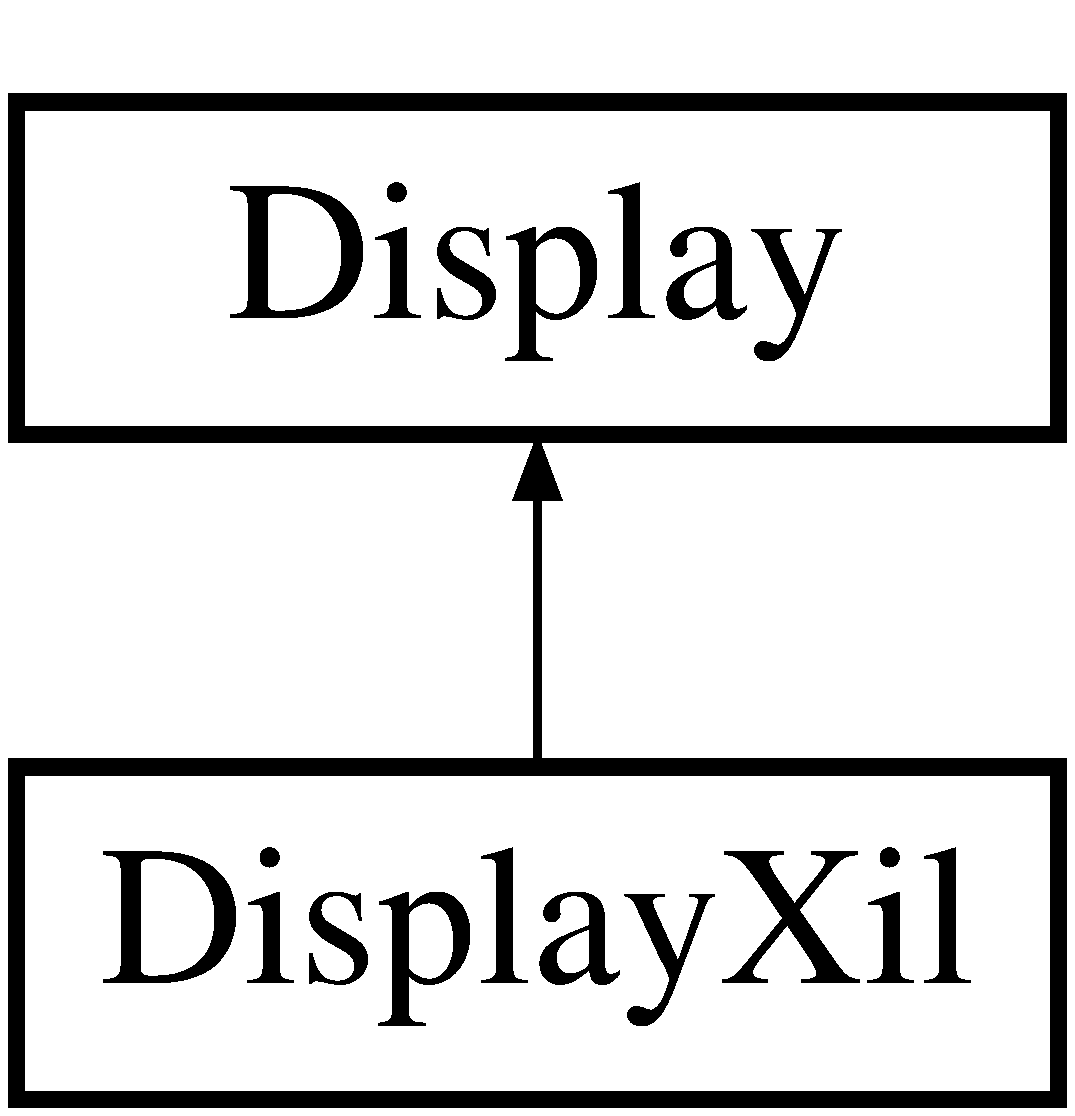
\includegraphics[height=2.000000cm]{class_display_xil}
\end{center}
\end{figure}
\subsection*{Public Member Functions}
\begin{DoxyCompactItemize}
\item 
\hypertarget{class_display_xil_acd2a25de77eefd27b250ff4503957064}{{\bfseries Display\+Xil} (\hyperlink{class_iic_ctrl}{Iic\+Ctrl} $\ast$)}\label{class_display_xil_acd2a25de77eefd27b250ff4503957064}

\item 
\hypertarget{class_display_xil_a6767d57ca04825ba2e4479912a068b2e}{virtual int {\bfseries \+\_\+initscr} ()}\label{class_display_xil_a6767d57ca04825ba2e4479912a068b2e}

\item 
\hypertarget{class_display_xil_adea353eaa49aa54254edb62bafcd6157}{virtual void {\bfseries \+\_\+clear} ()}\label{class_display_xil_adea353eaa49aa54254edb62bafcd6157}

\item 
\hypertarget{class_display_xil_ae6cb9b43498f469a41da87f36ee1690f}{virtual void {\bfseries \+\_\+endwin} ()}\label{class_display_xil_ae6cb9b43498f469a41da87f36ee1690f}

\item 
\hypertarget{class_display_xil_a9c62240b8933713ed3eb9dd877c609f8}{virtual void {\bfseries \+\_\+refresh} ()}\label{class_display_xil_a9c62240b8933713ed3eb9dd877c609f8}

\item 
\hypertarget{class_display_xil_a7f2623c14f9777af5d58805557acd48b}{virtual void {\bfseries \+\_\+getch} ()}\label{class_display_xil_a7f2623c14f9777af5d58805557acd48b}

\item 
\hypertarget{class_display_xil_ac110fd5b80fa314ec631cebe53322cdb}{virtual void {\bfseries \+\_\+addstr} (const char $\ast$)}\label{class_display_xil_ac110fd5b80fa314ec631cebe53322cdb}

\item 
\hypertarget{class_display_xil_ac14d60ce17eb29dd2b8f95c795f0ed1a}{virtual void {\bfseries \+\_\+move} (int, int)}\label{class_display_xil_ac14d60ce17eb29dd2b8f95c795f0ed1a}

\item 
\hypertarget{class_display_xil_aa49760c3485ac443c17e5aa22e5bdf58}{Xuint32 {\bfseries get\+Width} ()}\label{class_display_xil_aa49760c3485ac443c17e5aa22e5bdf58}

\item 
\hypertarget{class_display_xil_affa3b96c0ab1cacc7be57894d23ee775}{Xuint32 {\bfseries get\+Height} ()}\label{class_display_xil_affa3b96c0ab1cacc7be57894d23ee775}

\item 
\hypertarget{class_display_xil_a2b2d3013803ffa0b2516b9e5def7080c}{int {\bfseries get\+Resolution} ()}\label{class_display_xil_a2b2d3013803ffa0b2516b9e5def7080c}

\item 
\hypertarget{class_display_xil_ac2e2d2e53c6845c94826d66609051e4e}{Xuint32 {\bfseries get\+Hdmi\+Vtc\+Device\+Id} ()}\label{class_display_xil_ac2e2d2e53c6845c94826d66609051e4e}

\item 
\hypertarget{class_display_xil_a91b8aeef0fdc4d6e14f431851fe4d7d6}{Xuint32 {\bfseries get\+Hdmi\+Vdma\+Device\+Id} ()}\label{class_display_xil_a91b8aeef0fdc4d6e14f431851fe4d7d6}

\item 
\hypertarget{class_display_xil_ab693f7986ccb1086fde71d2fb96922a7}{Xuint32 {\bfseries set\+Hdmi\+Display\+Mem\+Base\+Addr} (Xuint32 addr)}\label{class_display_xil_ab693f7986ccb1086fde71d2fb96922a7}

\item 
\hypertarget{class_display_xil_ab760adbb64268a15b5988e1b62c5f424}{Xuint32 {\bfseries get\+Hdmi\+Display\+Mem\+Base\+Addr} ()}\label{class_display_xil_ab760adbb64268a15b5988e1b62c5f424}

\item 
\hypertarget{class_display_xil_a82995915d86cd698ca4c88078391af4e}{X\+Axi\+Vdma $\ast$ {\bfseries get\+Axi\+Vdma} ()}\label{class_display_xil_a82995915d86cd698ca4c88078391af4e}

\item 
\hypertarget{class_display_xil_a0e3fe7495568f5c5d0c75af7a6f3ac3f}{X\+Axi\+Vdma\+\_\+\+Dma\+Setup $\ast$ {\bfseries get\+Axi\+Vdma\+Cfg} ()}\label{class_display_xil_a0e3fe7495568f5c5d0c75af7a6f3ac3f}

\end{DoxyCompactItemize}


The documentation for this class was generated from the following files\+:\begin{DoxyCompactItemize}
\item 
/\+Users/neiljohnson/sandbox/agile-\/codev-\/platform/sw/src/Display\+Xil.\+h\item 
/\+Users/neiljohnson/sandbox/agile-\/codev-\/platform/sw/src/Display\+Xil.\+cpp\end{DoxyCompactItemize}

\hypertarget{class_drawing}{\section{Drawing Class Reference}
\label{class_drawing}\index{Drawing@{Drawing}}
}
\subsection*{Public Member Functions}
\begin{DoxyCompactItemize}
\item 
\hypertarget{class_drawing_a0c72054134258f0cc9faa0a28f29d8e6}{{\bfseries Drawing} (\hyperlink{class_board}{Board} $\ast$board, \hyperlink{class_display}{Display} $\ast$display)}\label{class_drawing_a0c72054134258f0cc9faa0a28f29d8e6}

\item 
\hypertarget{class_drawing_a3f871774278189f8fc0b0ee17dee9bb3}{bool {\bfseries is\+Initialized} (void)}\label{class_drawing_a3f871774278189f8fc0b0ee17dee9bb3}

\item 
\hypertarget{class_drawing_a6362cd3a4d223f6ce719bbe8a78e4678}{void {\bfseries refresh\+Drawing} (void)}\label{class_drawing_a6362cd3a4d223f6ce719bbe8a78e4678}

\item 
\hypertarget{class_drawing_a262442a8c5088a9d1a48e5fd3a727ac4}{void {\bfseries play} (int)}\label{class_drawing_a262442a8c5088a9d1a48e5fd3a727ac4}

\item 
\hypertarget{class_drawing_aedc140a5811f608a0ae0cc46e65a687e}{void {\bfseries initial\+Cell} (int, int)}\label{class_drawing_aedc140a5811f608a0ae0cc46e65a687e}

\item 
\hypertarget{class_drawing_a86076acc6d1bda3d3a0fc271c96fff62}{void {\bfseries initialize\+Board} (void)}\label{class_drawing_a86076acc6d1bda3d3a0fc271c96fff62}

\end{DoxyCompactItemize}


The documentation for this class was generated from the following files\+:\begin{DoxyCompactItemize}
\item 
/\+Users/neiljohnson/sandbox/agile-\/codev-\/platform/sw/src/Drawing.\+h\item 
/\+Users/neiljohnson/sandbox/agile-\/codev-\/platform/sw/src/Drawing.\+cpp\end{DoxyCompactItemize}

\hypertarget{class_iic_ctrl}{\section{Iic\+Ctrl Class Reference}
\label{class_iic_ctrl}\index{Iic\+Ctrl@{Iic\+Ctrl}}
}
\subsection*{Public Member Functions}
\begin{DoxyCompactItemize}
\item 
\hypertarget{class_iic_ctrl_af723bff67268b4eebcca42b0f20a352d}{{\bfseries Iic\+Ctrl} (u32 Hdmi\+I2c\+Base\+Addr=0)}\label{class_iic_ctrl_af723bff67268b4eebcca42b0f20a352d}

\item 
\hypertarget{class_iic_ctrl_a00fa06cc675dd562777bf5fd0831986a}{virtual int {\bfseries init} ()}\label{class_iic_ctrl_a00fa06cc675dd562777bf5fd0831986a}

\item 
\hypertarget{class_iic_ctrl_a86cecdf3f461a19fd77e1cdd2110a207}{virtual unsigned {\bfseries iic\+Write} (Xuint32, Xuint8, Xuint8 $\ast$, Xuint8)}\label{class_iic_ctrl_a86cecdf3f461a19fd77e1cdd2110a207}

\item 
\hypertarget{class_iic_ctrl_a297b5861772056204b83ce3f9037ea3c}{u32 {\bfseries get\+Hdmi\+I2c\+Base\+Addr} ()}\label{class_iic_ctrl_a297b5861772056204b83ce3f9037ea3c}

\end{DoxyCompactItemize}
\subsection*{Static Public Attributes}
\begin{DoxyCompactItemize}
\item 
\hypertarget{class_iic_ctrl_a14fca6591db47dd1c8f371b0cff29284}{static Xuint8 {\bfseries carrier\+\_\+hdmi\+\_\+out\+\_\+config} \mbox{[}C\+A\+R\+R\+I\+E\+R\+\_\+\+H\+D\+M\+I\+\_\+\+O\+U\+T\+\_\+\+C\+O\+N\+F\+I\+G\+\_\+\+L\+E\+N\mbox{]}\mbox{[}3\mbox{]}}\label{class_iic_ctrl_a14fca6591db47dd1c8f371b0cff29284}

\end{DoxyCompactItemize}


The documentation for this class was generated from the following files\+:\begin{DoxyCompactItemize}
\item 
/\+Users/neiljohnson/sandbox/agile-\/codev-\/platform/sw/src/Iic\+Ctrl.\+h\item 
/\+Users/neiljohnson/sandbox/agile-\/codev-\/platform/sw/src/Iic\+Ctrl.\+cpp\end{DoxyCompactItemize}

\hypertarget{structstruct__vres__timing__t}{\section{struct\+\_\+vres\+\_\+timing\+\_\+t Struct Reference}
\label{structstruct__vres__timing__t}\index{struct\+\_\+vres\+\_\+timing\+\_\+t@{struct\+\_\+vres\+\_\+timing\+\_\+t}}
}
\subsection*{Public Attributes}
\begin{DoxyCompactItemize}
\item 
\hypertarget{structstruct__vres__timing__t_a55c4484970db9927eee66daa71c9cab1}{char $\ast$ {\bfseries p\+Name}}\label{structstruct__vres__timing__t_a55c4484970db9927eee66daa71c9cab1}

\item 
\hypertarget{structstruct__vres__timing__t_a386ae8ea8b832e15381edcaee7ac68fe}{Xuint32 {\bfseries V\+Active\+Video}}\label{structstruct__vres__timing__t_a386ae8ea8b832e15381edcaee7ac68fe}

\item 
\hypertarget{structstruct__vres__timing__t_afa1898449359597f9339c1d5327e4f71}{Xuint32 {\bfseries V\+Front\+Porch}}\label{structstruct__vres__timing__t_afa1898449359597f9339c1d5327e4f71}

\item 
\hypertarget{structstruct__vres__timing__t_a1c328bb23b67368cfe4190f10361020d}{Xuint32 {\bfseries V\+Sync\+Width}}\label{structstruct__vres__timing__t_a1c328bb23b67368cfe4190f10361020d}

\item 
\hypertarget{structstruct__vres__timing__t_a8d7253257bfe8b55466a48f652608260}{Xuint32 {\bfseries V\+Back\+Porch}}\label{structstruct__vres__timing__t_a8d7253257bfe8b55466a48f652608260}

\item 
\hypertarget{structstruct__vres__timing__t_a394ebb85a22a21bba3ace63e188eebd1}{Xuint32 {\bfseries V\+Sync\+Polarity}}\label{structstruct__vres__timing__t_a394ebb85a22a21bba3ace63e188eebd1}

\item 
\hypertarget{structstruct__vres__timing__t_ad8174a45fb1ca9230ec34120f19af2a6}{Xuint32 {\bfseries H\+Active\+Video}}\label{structstruct__vres__timing__t_ad8174a45fb1ca9230ec34120f19af2a6}

\item 
\hypertarget{structstruct__vres__timing__t_af9a6949826053d49500462fb1976631e}{Xuint32 {\bfseries H\+Front\+Porch}}\label{structstruct__vres__timing__t_af9a6949826053d49500462fb1976631e}

\item 
\hypertarget{structstruct__vres__timing__t_ae6665d9f5eef3d1f7ebc2b0c641c06e7}{Xuint32 {\bfseries H\+Sync\+Width}}\label{structstruct__vres__timing__t_ae6665d9f5eef3d1f7ebc2b0c641c06e7}

\item 
\hypertarget{structstruct__vres__timing__t_ac6c0f2fee41b82fbd0a0f7d9de16d979}{Xuint32 {\bfseries H\+Back\+Porch}}\label{structstruct__vres__timing__t_ac6c0f2fee41b82fbd0a0f7d9de16d979}

\item 
\hypertarget{structstruct__vres__timing__t_ad2e48b09dc45215820ea24697cf435a6}{Xuint32 {\bfseries H\+Sync\+Polarity}}\label{structstruct__vres__timing__t_ad2e48b09dc45215820ea24697cf435a6}

\end{DoxyCompactItemize}


The documentation for this struct was generated from the following file\+:\begin{DoxyCompactItemize}
\item 
/\+Users/neiljohnson/sandbox/agile-\/codev-\/platform/sw/src/video\+\_\+resolution.\+h\end{DoxyCompactItemize}

%--- End generated contents ---

% Index
\newpage
\phantomsection
\addcontentsline{toc}{chapter}{Index}
\printindex

\end{document}
